
\chapter{Observer Based Controls}
\label{chap:ObserverBasedControls}

Chapter \ref{chap:UNHTableSat1A} detailed how TableSat's sensor readings could be quantified and represented in terms of engineering units.  Chapter \ref{chap:SatelliteAttitudeModeling} established the state representation of the system and the chosen dynamic equations used to model it's behavior.  This chapter will focus on the estimation techniques to improve the accuracy of the state representations, and control techniques to guide the system into the desired state.

\section{State Error}
\label{sec:StateError}

In both the estimation and control techniques, a process for determining how close two states are from each other is required.  For the estimation case,  the error $\bs{\hat{x}}_e$ between the measured state $\bs{x}$ and the estimated state $\bs{\hat{x}}$.  For the controllers, the state error $\bs{x}_e$ representing the offset between the estimated state $\bs{\hat{x}}$ and the desired state $\bs{x}_d$.

\begin{subequations}
  \begin{align}
    \bs{\hat{x}}_e &= \bs{\hat{x}} - \bs{x} \\
    \bs{x}_e &= \bs{\hat{x}} - \bs{x}_d
  \end{align}
  \label{eqn:StateError}
\end{subequations}

Multiple methods were used to quantify the differences in states.  For comparison and to demonstrate their use with TSatPy, the following sections will limit its focus on a single update of proportional estimator.

\begin{equation}
  \bs{\hat{x}(t_{k+1})} = \bs{\hat{x}}(t_{k}) + \bs{K_p} ( \bs{\hat{x}}(t_{k}) - \bs{x}(t_{k}) )
  \label{eqn:PEstimatorStateDiff}
\end{equation}

This simple estimation technique has some notable deficiencies when applied to the attitude parameters of a spin stabilized satellite.  These parameters are expected to change as the satellite rotates, but this model has no method for predicting the change in parameters so will rely solely on the state error to correct $\bs{\hat{x}(t_{k+1})}$.  After an adequate method is established for calculating the state error, later sections will address improving upon the proportional estimator.

The sample error calculation in this section will be based off a last estimated state, $\bs{\hat{x}}(t_{k})$, of a $190^o$ rotation about $+z$-axis and a body rate of $\omega_z = 3$ rad/sec.  The associated the measured state, $\bs{x}(t_{k})$, is a $44^o$ rotation about the axis $0 \bs{i} + 0.1 \bs{j} + 1\bs{k}$ and a body rate of $\omega_z = 3.1$ rad/sec.


\begin{subequations}
  \begin{align}
    \bs{\hat{x}}(t_{k})
    = \begin{bmatrix}  \bs{\hat{q}}(t_{k}) \\ \bs{\hat{\omega}}(t_{k}) \end{bmatrix}
    &= \begin{bmatrix} 0 \bs{i} +0 \bs{j} -0.996195 \bs{k} -0.0871557 \\ 0 \bs{i} +0 \bs{j} +3 \bs{k} \end{bmatrix}\\
    \bs{x}(t_{k})
    = \begin{bmatrix}  \bs{q}(t_{k}) \\ \bs{\omega}(t_{k}) \end{bmatrix}
    &= \begin{bmatrix} 0 \bs{i} -0.0372747 \bs{j} -0.372747 \bs{k} +0.927184 \\ 0 \bs{i} +0 \bs{j} +3.1 \bs{k} \end{bmatrix}
  \end{align}
  \label{eqn:StateDifferenceQuaternionSamples}
\end{subequations}

\begin{singlespace}
  \begin{minted}[mathescape,linenos,numbersep=10pt,frame=lines,framesep=2mm]{python}
from TSatPy.State import Quaternion, QuaternionError, State, BodyRate
import numpy as np

x_hat = State(
    Quaternion([0,0,1],radians=190/180.0*np.pi),
    BodyRate([0,0,3]))
x_m = State(
    Quaternion([0,0.1,1],radians=44/180.0*np.pi),
    BodyRate([0,0,3.1]))
print("x_hat:  %s" % (x_hat))
print("x_m:    %s" % (x_m))

# Prints Out
# x_hat:  <Quaternion [-0 -0 -0.996195], -0.0871557>,
#         <BodyRate [0 0 3]>
# x_m:    <Quaternion [-0 -0.0372747 -0.372747], 0.927184>,
#         <BodyRate [0 0 3.1]>
  \end{minted}
\nocite{minted}
\end{singlespace}

Section \ref{subsec:StateDifference} will start out with the standard element wise matrix difference to represent the state error.

\subsection{State Difference}
\label{subsec:StateDifference}

The standard method for calculating the state error in either an estimation or control method is to calculate an element-wise difference.  TableSat has a seven element state in matrix form and expanding Equation \ref{eqn:StateError} becomes

\begin{equation}
  \begin{aligned}
    \bs{\hat{x}}_e(t_{k}) &= \begin{bmatrix}  \bs{\hat{q}}_e(t_{k}) \\ \bs{\hat{\omega}}_e(t_{k}) \\ \end{bmatrix} \\
    &= \begin{bmatrix} (\hat{q}_1 - q_{1}) \bs{i} + (\hat{q}_2 - q_{2}) \bs{j} + (\hat{q}_3 - q_{3}) \bs{k} + \hat{q}_0 - q_{0} \\ (\hat{\omega}_x - \omega_{x}) \bs{i} + (\hat{\omega}_y - \omega_{y}) \bs{j} + (\hat{\omega}_z - \omega_{z}) \bs{k} \end{bmatrix}
  \end{aligned}
  \label{eqn:StateDifference}
\end{equation}


Calculating the difference between the example estimated and measured states in Equation \ref{eqn:StateDifferenceQuaternionSamples} yields a state difference of

\begin{equation}
  \begin{aligned}
    \bs{\hat{x}}_e(t_{k})
    = \begin{bmatrix}  \bs{\hat{q}}_e(t_{k}) \\ \bs{\hat{\omega}}_e(t_{k}) \end{bmatrix}
    &= \begin{bmatrix} 0 \bs{i} +0.0372747 \bs{j} -0.623447 \bs{k} -1.01434 \\ 0 \bs{i} +0 \bs{j} -0.1 \bs{k} \end{bmatrix}
  \end{aligned}
  \label{eqn:StateDifferenceSample}
\end{equation}


\begin{singlespace}
  \begin{minted}[mathescape,linenos,numbersep=10pt,frame=lines,framesep=2mm]{python}
x_e = State(
    Quaternion(x_hat.q.vector - x_m.q.vector,
        x_hat.q.scalar - x_m.q.scalar),
    x_hat.w - x_m.w)
print("x_e:  %s" % (x_e))

# Prints Out
# x_e:  <Quaternion [0 0.0372747 -0.623447], -1.01434>,
#       <BodyRate [0 0 -0.1]>
  \end{minted}
\nocite{minted}
\end{singlespace}


The body rate error calculations are well behaved and are able to be directly used with standard estimation based control techniques.  The difference in quaternion parameters however pose a number of problems even when used in a basic proportional estimator.  Using this method of error measurement will be difficult especially since after a cursory review the scalar quantity in the error quaternion that is outside the possible range for a rotational quaternion.  Section \ref{subsec:QuaternionDifferencebasedPEstimator} will attempt to use this state difference along with a standard proportional estimation technique.

\subsection{Quaternion Difference based P-Estimator}
\label{subsec:QuaternionDifferencebasedPEstimator}

Taking the quaternion difference from Equation \ref{eqn:StateDifferenceSample}, and incorporating into the proportional estimation correction in Equation \ref{eqn:PEstimatorStateDiff} produces an state adjustment and estimated attitude of

\begin{equation}
  \begin{aligned}
    \bs{q}_{adj} = -0.8 \cdot \bs{q}_e =& -0.8 \cdot (0 \bs{i} + 0.0372747 \bs{j} -0.623447 \bs{k} -1.01434 ) \\
                       =& 0 \bs{i} -0.0298198 \bs{j} +0.498758 \bs{k} +0.811472 \\
    \bs{\hat{q}(t_{k+1})} =& \bs{\hat{q}(t_{k})} + \bs{q}_{adj} \\
                       =& 0 \bs{i} -0.0298198 \bs{j} -0.497437 \bs{k} + 0.724316 \\
  \end{aligned}
\end{equation}

\begin{singlespace}
  \begin{minted}[mathescape,linenos,numbersep=10pt,frame=lines,framesep=2mm]{python}
q_hat = x_hat.q
q_e = x_e.q
q_adj = Quaternion(-0.8 * q_e.vector, -0.8 * q_e.scalar)
q_hat_new = Quaternion(q_hat.vector + q_adj.vector,
        q_hat.scalar + q_adj.scalar)

print("q_e:         %s" % (q_e))
print("q_adj:       %s" % (q_adj))
print("q_hat_new:   %s" % (q_hat_new))
print("|q_hat_new|: %g" % (q_hat_new.mag))

# Prints Out
# q_e:         <Quaternion [0 0.0372747 -0.623447], -1.01434>
# q_adj:       <Quaternion [-0 -0.0298198 0.498758], 0.811472>
# q_hat_new:   <Quaternion [-0 -0.0298198 -0.497437], 0.724316>
# |q_hat_new|: 0.879185
  \end{minted}
\nocite{minted}
\end{singlespace}

The new estimate for the quaternion attitude has been adjusted closer to the measured state although the newly estimated state has a norm of $ \| \bs{\hat{q}(t_{k+1})} \| = 0.879185$.  Since failing to conform to the unit magnitude for rotational quaternions, this newly estimated attitude quaternion corrupts the systems state especially over multiple steps and long simulations.  For rotational quaternions with norms less that the unit quaternion the rotated points end up converging into the origin.  If the adjustment ends up with a rotational quaternion larger than a unit magnitude, rotated points dilate away from the origin.

\begin{singlespace}
  \begin{minted}[mathescape,linenos,numbersep=10pt,frame=lines,framesep=2mm]{python}
pt = np.mat([[1,0,0]])
pt = q_hat_new.rotate_points(pt)
print("pt * pt.T:   %s" % (pt * pt.T))

# Prints Out
# pt * pt.T:   [[ 0.5974769]]
  \end{minted}
\nocite{minted}
\end{singlespace}


\subsection{Scaled Quaternion Difference based P-Estimator}
\label{sec:ScaledQuaternionDifferencebasedPEstimator}

The next step to correct for the dilation or compression of points is to scale the adjusted quaternion to a unit quaternion before using it to represent the system's state.  The quaternion can be scaled through a standard vector normalization.

\begin{equation}
  \bs{\hat{q}}_n = \frac{\bs{q}_v + q_0}{\sqrt{\bs{q}_v \bullet \bs{q}_v + q_0^2}}
  \label{eqn:NormalizeQuaternion}
\end{equation}

\begin{singlespace}
  \begin{minted}[mathescape,linenos,numbersep=10pt,frame=lines,framesep=2mm]{python}
print("q_hat_new:   %s" % (q_hat_new))
q_hat_new.normalize()
print("q_hat_new:   %s" % (q_hat_new))
print("|q_hat_new|: %g" % (q_hat_new.mag))

# Prints Out
# q_hat_new:   <Quaternion [-0 -0.0298198 -0.497437], 0.724316>
# q_hat_new:   <Quaternion [-0 -0.0339175 -0.565793], 0.823849>
# |q_hat_new|: 1
  \end{minted}
\nocite{minted}
\end{singlespace}

The newly estimated state is equivalent to a $69$ degree rotation about
\begin{equation}\hat{\bs{e}} = \begin{bmatrix} 0 & -0.0598395 & -0.998208 \end{bmatrix}\end{equation}.  While this state estimate conforms to the unit quaternion requirement and will no longer corrupt rotations, it has little in common with the desired $0.8$ proportional gain used the estimator's design.

\begin{singlespace}
  \begin{minted}[mathescape,linenos,numbersep=10pt,frame=lines,framesep=2mm]{python}
e, r = q_hat_new.to_rotation()
print("e: <%g, %g, %g>\ndegree: %g" % (
    e[0,0],e[1,0],e[2,0], r * 180.0 / np.pi))

# Prints Out
# e: <-0, -0.0598395, -0.998208>
# degree: 69.056
  \end{minted}
\nocite{minted}
\end{singlespace}


\subsection{Quaternion Multiplicative Correction}
\label{subsec:QuaternionMultiplicativeCorrection}

The previous sections have established that the state difference approach for adjusting for errors in attitude measurements has significant issues especially for low frequency updates with high error values.  The quaternion multiplication defined in Equation \ref{eqn:QuaternionMultiplication} can be used to modify the attitude while not introducing corruption into the model if used with rotational unit quaternions.

If the estimated and measured states converge with the multiplicative correction, the error quaternion should converge to the identity quaternion.  The identity quaternion as with the identity matrix is the quantity that when multiplied by another quaternion, does not modify its value.  This identity holds true for general as well as rotational quaternions.

\begin{equation}
  \bs{q}_I = 0 \bs{i} + 0 \bs{j} + 0 \bs{k} + 1
\end{equation}

An Identity function was created it the TSatPy.State module to construct an identity quaternion.

\begin{singlespace}
  \begin{minted}[mathescape,linenos,numbersep=10pt,frame=lines,framesep=2mm]{python}
from TSatPy import State

q = State.Quaternion([1,2,3], 4)
print("q       = %s" % q)
q_I = State.Identity()
print("q_I     = %s" % q_I)
print("q_I * q = %s" % (q_I * q))

# Prints Out
# q       = <Quaternion [1 2 3], 4>
# q_I     = <Quaternion [0 0 0], 1>
# q_I * q = <Quaternion [1 2 3], 4>
  \end{minted}
  \nocite{minted}
\end{singlespace}

Rotational quaternions are considered equal if they represent the same attitude.  The same attitude can be represented by more than one distinct quaternions, so a strict equality is not adequate.  The test for equality can be done by using the quaternion conjugate $\bs{q}^*$.

\begin{subequations}
  \begin{align}
    \bs{\hat{q}} = \bs{q} & \iff \bs{\hat{q}}^* \otimes \bs{q} = \bs{q}^* \otimes \bs{\hat{q}} = \bs{q}_I \text{ or } -\bs{q}_I \\
    \text{where } \bs{q}^* &= \begin{bmatrix} -\bs{v} \\ q_0 \end{bmatrix}
  \end{align}
  \label{eqn:QuaternionEquality}
\end{subequations}

The sample below shows how two distinct quaternions can represent the same attitude and that Equation \ref{eqn:QuaternionEquality} holds true.

\begin{singlespace}
  \begin{minted}[mathescape,linenos,numbersep=10pt,frame=lines,framesep=2mm]{python}
a = Quaternion([0,0,1],radians=190/180.0*np.pi)
b = Quaternion([0,0,1],radians=(190 + 360)/180.0*np.pi)

print("a:          %s" % (a))
print("b:          %s" % (b))
print("a.conj * b: %s" % (a.conj * b))

# Prints Out
# a:          <Quaternion [-0 -0 -0.996195], -0.0871557>
# b:          <Quaternion [0 0 0.996195], 0.0871557>
# a.conj * b: <Quaternion [0 0 -3.46945e-16], -1>
  \end{minted}
\nocite{minted}
\end{singlespace}

Equation \ref{eqn:QuaternionEquality} provides a method for determining whether two quaternions represent the same attitude, it can also be used to quantify the difference between two rotational quaternions using the multiplicative comparison.

\begin{equation}
  \bs{q}_e = \bs{q}^* \otimes \bs{\hat{q}}
  \label{eqn:QuaternionError}
\end{equation}

Continuing with the example measured and estimated states from Equation \ref{eqn:StateDifferenceQuaternionSamples}, the multiplicative quaternion error between these states evaluates to

\begin{equation}
  \begin{aligned}
    \bs{q}_e = & \bs{q}^* \otimes \bs{\hat{q}} \\
    = & \big( 0 \bs{i} -0.0372747 \bs{j} -0.372747 \bs{k} +0.927184 \big)^* \\
    & \otimes \big( 0 \bs{i} +0 \bs{j} -0.996195 \bs{k} -0.0871557 \big)\\
    = & -0.0371329 \bs{i} -0.00324871 \bs{j} -0.956143 \bs{k} +0.29052
  \end{aligned}
  \label{eqn:QuaternionErrorSample}
\end{equation}

The sample error measurement in Equation \ref{eqn:QuaternionErrorSample} relates well to the deviations in the estimated and measured attitudes as it represents a 146 degree rotation about the Euler axis $<-0.0388067, -0.00339514, -0.999241>$ which would rotate the estimated quaternion back to match up perfectly with the measured state.  The multiplicative error correction quaternion also solves the issue encountered in Section \ref{subsec:QuaternionDifferencebasedPEstimator} where the magnitude of the error quaternion did not remain fixed at the unit quaternion.

\begin{singlespace}
  \begin{minted}[mathescape,linenos,numbersep=10pt,frame=lines,framesep=2mm]{python}
from TSatPy.State import QuaternionError
q_e = QuaternionError(x_hat.q, x_m.q)

print("q_e:   %s" % (q_e))
print("|q_e|: %s" % (q_e.mag))
e, r = q_e.to_rotation()
print("e:     <%g, %g, %g>\ndegree: %g" % (
    e[0,0],e[1,0],e[2,0], r * 180.0 / np.pi))

# Prints Out
# q_e:   <Quaternion [-0.0371329 -0.00324871 -0.956143], 0.29052>
# |q_e|: 1.0
# e:     <-0.0388067, -0.00339514, -0.999241>
# degree: 146.222
  \end{minted}
\nocite{minted}
\end{singlespace}

\subsection{Quaternion Multiplicative Correction P-Estimation}
\label{subsec:QuaternionMultiplicativeCorrectionPEstimation}

Section \ref{subsec:QuaternionMultiplicativeCorrection} was able to establish a method for quantifying differences in attitudes in a method that preserves the integrity of the rotational quaternion while creating a representative measure of the state error.  For the next step, a series of options were investigated to determine how the error measurement can be used in estimation and control techniques.

\subsubsection{Parameter Multiplier}
\label{subsubsec:ParameterMultiplier}

With a parameter multiplier method, the four parameters of the error quaternion get scaled by a $\bs{K_p}$ term similar to the standard proportional adjustment.

\begin{equation}
  \bs{q}_{adj} = \bs{K_p} \bs{q}_e
    = \bs{K_p} \begin{bmatrix} \bs{v}_e \\ q_{e0} \end{bmatrix}
    = \begin{bmatrix} \bs{K_{vp}}\bs{v}_e \\ K_{0p} \cdot q_{e0} \end{bmatrix}
  \label{eqn:ParameterMultiplier}
\end{equation}

The $\bs{K_{vp}}$ term is a 3x3 matrix.  Since $\bs{v}_e$ defines the path between the estimated and measured quaternions the only form of $\bs{K_{vp}}$ that would not corrupt the direction mapped between the two states is

\begin{equation}
  \bs{K_{vp}} \bs{v}_e = \lambda \bs{v}_e
  \label{eqn:QuaternionVectorCorrection}
\end{equation}

The effect of the $\lambda$ parameter is to modify the magnitude of the quaternion's Euler axis but not modify it's direction.  Combining \ref{eqn:QuaternionVectorCorrection} with \ref{eqn:ParameterMultiplier} yields

\begin{equation}
  \bs{q}_{adj} = \begin{bmatrix} \lambda \bs{v}_e \\ K_{0p} \cdot q_{e0} \end{bmatrix}
  \label{eqn:QuaternionScalarMultiplier}
\end{equation}

Reducing the tunable parameters for the proportional quaternion estimator to $\lambda$ and $K_{0p}$.  This configuration, shares the same flaws as the state difference approach in Section \ref{subsec:QuaternionDifferencebasedPEstimator} where the magnitude of the adjusted quaternion can vary from the unit quaternion causing dilation or compression of rotated points.

\begin{singlespace}
  \begin{minted}[mathescape,linenos,numbersep=10pt,frame=lines,framesep=2mm]{python}
q_adj = Quaternion(
    q_e.vector * 0.7,  # lambda chosen as 0.7
    q_e.scalar * 0.4)  # K_p0 chosen as 0.4

print("q_adj:   %s" % (q_adj))
print("|q_adj|: %s" % (q_adj.mag))

# Prints Out
# q_adj:   <Quaternion [-0.025993 -0.0022741 -0.6693], 0.116208>
# |q_adj|: 0.679814272084
  \end{minted}
\nocite{minted}
\end{singlespace}


\subsubsection{Normalized Parameter Multiplier}
\label{subsubsec:NormalizedParameterMultiplier}

Normalizing the paramater multiplier's adjustment quaternion resolves the issues with dilating and contracting points as it did in Section \ref{sec:ScaledQuaternionDifferencebasedPEstimator}.  A normalized parameter multiplier quaternion does not suffer from an invalid Euler axis of rotation as in Section \ref{sec:ScaledQuaternionDifferencebasedPEstimator} as only the magnitude of the quaternion's vector is modified.  The scalar quantity however still ends up being muddied due to the coupling between  and $K_{0p}$ that occurs via normalization.  A constant angular error and $K_{0p}$ can create varied adjustment values based on the selection of the $\lambda$ gain.

\subsubsection{Scalar Multiplier with Normalization}
\label{subsubsec:ScalarMultiplierWithNormalization}

Since the $\lambda$ gain used above provides no benefit and only ends up complicating the quaternion adjustment calculation, it can be dropped leaving a quaternion adjustment based solely on a modification of the scalar quantity.  After the scalar gain $k$, the quaternion can be normalized back to a unit quaternion.

\begin{equation}
  \begin{aligned}
  \bs{q}_{adj} = & \begin{bmatrix} \bs{v}_e / \alpha \\ ( k \cdot q_{e0} )  / \alpha \end{bmatrix} \\
  \text{where } \alpha & = \sqrt{\bs{v}_e^T \cdot \bs{v}_e + k^2 \cdot q_{e0}^2}
  \end{aligned}
  \label{eqn:ScalarMultiplierWithNormalization}
\end{equation}

Equation \ref{eqn:ScalarMultiplierWithNormalization} has a few strengths when used to apply adjustments to a quaternion attitude estimate.  It's based off the multiplicative correction quaternion that accurately quantifies the difference in estimated and measured states.  The normalization ensures that the rotational quaternion representation is not corrupted and when applied will not cause dilation or compression of the model.

The disadvantage to using this representation is that the quaternion scalar parameter is a nonlinear function of the rotation angle (Equation \ref{eqn:RotationalQuaternionDefinition}).  Applying a constant scalar multiplier to it will result in inconsistent adjustment amount depending on the position along the sinusoidal value.

\subsubsection{Angle Multiplier with Vector Magnitude Normalization}
\label{subsubsec:AngleMultiplierWithVectorMagnitudeNormalization}

The section will cover the final version of the quaternion adjustment calculation that takes into consideration all the issues encountered in the above sections.  The function designated in this thesis for the scaling of a quaternion to for use with quaternion multiplicative corrections while maintaining it's connection to the physical system will be $\bs{\psi}(\bs{q}, k)$ where

\begin{equation}
  \begin{aligned}
    \bs{\psi}(\bs{q}, k) &= \begin{bmatrix} \bs{v} / \gamma \\ \cos ( k \cdot \cos^{-1} (q_0))  \end{bmatrix} \\
    \text{where } \gamma &= \sqrt{\frac{\bs{v}^T \cdot \bs{v}}{\sin^2 ( k \cdot \cos^{-1} (q_0))}} \\
    \bs{q} &= \begin{bmatrix} \bs{v} \\ q_0  \end{bmatrix}
  \end{aligned}
  \label{eqn:PSI}
\end{equation}

Using Equation \ref{eqn:PSI} to create a rotational quaternion adjustment for the proportional estimator would take the form.

\begin{equation}
  \bs{q}_{adj} = \bs{\psi}(\bs{q}_e, k)
  \label{eqn:PEstimatorAngleMultiplierwithVectorMagnitudeNormalization}
\end{equation}

The code snippet below demonstrates the usage of Equation \ref{eqn:PEstimatorAngleMultiplierwithVectorMagnitudeNormalization} with TSatPy.  The proposed error between the measured and estimated quaternions is constructed as a $45^o$ rotation about the body's $z$-axis.  With a chosen gain of 0.2, the expected quaternion adjustment is correct in evaluating to be a $9^o$ rotation about the $z$-axis that still conforms to the unit norm of a rotational quaternion.

\begin{singlespace}
  \begin{minted}[mathescape,linenos,numbersep=10pt,frame=lines,framesep=2mm]{python}
from TSatPy.State import Quaternion
import numpy as np

k = 0.2
degree = 45

q_e = Quaternion([0,0,1], radians=degree/180.0*np.pi)
print("q_e:     %s" % (q_e))

kpc = k * np.arccos(q_e.scalar)
gamma = np.sqrt((q_e.vector.T * q_e.vector)[0,0] / (np.sin(kpc))**2)

q_adj = Quaternion(
    q_e.vector / gamma,
    np.cos(kpc))
print("q_adj:   %s" % (q_adj))
print("|q_adj|: %s" % (q_adj.mag))

e, r = q_adj.to_rotation()
print("e:       <%g, %g, %g>\ndegree: %g" % (
    e[0,0],e[1,0],e[2,0], r * 180.0 / np.pi))

# Prints Out
# q_e:     <Quaternion [-0 -0 -0.382683], 0.92388>
# q_adj:   <Quaternion [-0 -0 -0.0784591], 0.996917>
# |q_adj|: 1.0
# e:       <-0, -0, -1>
# degree: 9
  \end{minted}
\nocite{minted}
\end{singlespace}

\subsection{Representative State Adjustments}
\label{subsec:RepresentativeStateAdjustments}

The work described in Sections \ref{subsec:StateDifference} through \ref{subsubsec:AngleMultiplierWithVectorMagnitudeNormalization} have established a solid foundation to quantify the state error along with appropriate methods for scaling state errors.

Quaternion Error

\begin{equation}
  \bs{q}_e = \bs{q}^* \otimes \bs{\hat{q}}
\end{equation}

Adjustment Quaternions

\begin{equation}
  \begin{aligned}
    \bs{q}_{adj} &= \bs{\psi}(\bs{q}_e, K_{qp}) \\
    \text{where } \bs{\psi}(\bs{q}, k) &= \begin{bmatrix} \bs{v} / \gamma \\ \cos ( k \cdot \cos^{-1} (q_0))  \end{bmatrix} \\
    \gamma &= \sqrt{\frac{\bs{v}^T \cdot \bs{v}}{\sin^2 ( k \cdot \cos^{-1} (q_0))}} \\
    \bs{q} &= \begin{bmatrix} \bs{v} \\ q_0  \end{bmatrix}
  \end{aligned}
\end{equation}

Body Rate Error

\begin{equation}
  \bs{\omega}_e = \bs{\hat{\omega}} - \bs{\omega}
\end{equation}

Adjustment Body Rates

\begin{equation}
  \bs{\omega}_{adj} = \bs{K_{\omega p}} \bs{\omega}_e
\end{equation}

The following snippet will demonstrate the implementation of the chosen state parameterization and correction methods.  The state is created to represent a 44 degree rotation about the body's $z$-axis with body rates of $\omega_x, \omega_y, \omega_z = 0.02, -0.04, 0.3$ rad/sec.  The corrected state will take $1/4$ of the quaternion rotation and scale the body rates by 0.2, 0.3, and 0.8 respectively.

\begin{singlespace}
  \begin{minted}[mathescape,linenos,numbersep=10pt,frame=lines,framesep=2mm]{python}
from TSatPy.State import State, Quaternion, BodyRate
from TSatPy.StateOperators import QuaternionGain, BodyRateGain, StateGain
import numpy as np

k_q = 0.25
k_w = [[0.2,0,0],[0,0.3,0],[0,0,0.8]]

x = State(
    Quaternion([0,0,1],radians=44/180.0*np.pi),
    BodyRate([0.02,-0.04,0.3]))
print("x:      %s" % (x))

Kx = StateGain(
    QuaternionGain(k_q),
    BodyRateGain(k_w))
print("Kx:     %s" % (Kx))

x_adj = Kx * x
print("x_adj:  %s" % (x_adj))

e, r = x_adj.q.to_rotation()
print("e:      <%g, %g, %g>\ndegree: %g" % (
    e[0,0],e[1,0],e[2,0], r * 180.0 / np.pi))

# Prints Out
# x:      <Quaternion [-0 -0 -0.374607], 0.927184>,
#         <BodyRate [0.02 -0.04 0.3]>
# Kx:     <StateGain <Kq 0.25>,
#           <Kw = [[ 0.2 0. 0. ] [ 0. 0.3 0. ] [ 0. 0. 0.8]]>>
# x_adj:  <Quaternion [-0 -0 -0.0958458], 0.995396>,
#         <BodyRate [0.004 -0.012 0.24]>
# e:      <-0, -0, -1>
# degree: 11
  \end{minted}
\nocite{minted}
\end{singlespace}


\section{Estimators}
\label{sec:Estimators}

Section \ref{sec:StateError} explained the rationale for the state representations and how adjustments can be applied to them in a manner than preserves the integrity of it's connection to the TableSat/MMS's physical orientation.  Usage of the gains are also done to make the effects of gain tuning more intuitive.

\subsection{PID Estimation}
\label{subsec:PIDEstimation}

This section will cover the use of PID adjustments to track state estimation.  Section \ref{sec:StateError} covered how states and especially the quaternion portion can be scaled.  The same method can be applied to the proportional part of the PID estimator.

\subsubsection{Proportional Estimator}
\label{subsubsec:ProportionalEstimator}

The proportional estimator defined in Equation \ref{eqn:PEstimator} was implemented in TSatPy.  Taking the estimated and measured states from Equation \ref{eqn:StateDifferenceQuaternionSamples}, an update of the TableSat/MMS state estimate is performed in the following manner.

\begin{subequations}
  \begin{align}
    \bs{\hat{x}}(t_{k+1}) &= \begin{bmatrix} \bs{\hat{q}}(t_{k+1}) \\ \bs{\hat{\omega}}(t_{k+1}) \end{bmatrix} \\
    \bs{\hat{q}}(t_{k+1}) &= \bs{\psi}(\bs{q}_e(t_{k}), K_{qp}) \otimes \bs{\hat{q}}(t_{k}) \\
    \bs{\hat{\omega}}(t_{k+1}) &= \bs{\hat{\omega}}(t_{k}) + \bs{K}_{\omega p} \cdot \bs{\omega}_e(t_{k})
  \end{align}
  \label{eqn:PEstimator}
\end{subequations}

\begin{singlespace}
  \begin{minted}[mathescape,linenos,numbersep=10pt,frame=lines,framesep=2mm]{python}
from TSatPy import StateOperators, Estimator, State
from TSatPy.Clock import Metronome
import numpy as np

x_ic = State.State(
    State.Quaternion([0,0,1],radians=190/180.0*np.pi),
    State.BodyRate([0,0,3]))
print("x_ic:    %s" % (x_ic))

k = 0.2
Kp = StateOperators.StateGain(
    StateOperators.QuaternionGain(k),
    StateOperators.BodyRateGain(np.eye(3) * k))
print("Kp:  %s" % (Kp))

c = Metronome()
pid = Estimator.PID(c, ic=x_ic)
pid.set_Kp(Kp)
print("pid: %s" % (pid))

x_m = State.State(
    State.Quaternion([0,0.1,1],radians=44/180.0*np.pi),
    State.BodyRate([0,0,3.1]))
pid.update(x_m)
print("pid.x_hat:   %s" % (pid.x_hat))

e, r = pid.x_hat.q.to_rotation()
print("e:      <%g, %g, %g>\ndegree: %g" % (
    e[0,0],e[1,0],e[2,0], r * 180.0 / np.pi))

# Prints Out
# x_ic:    <Quaternion [-0 -0 -0.996195], -0.0871557>,
#          <BodyRate [0 0 3]>
# Kp:  <StateGain <Kq 0.2>,
#      <Kw = [[ 0.2 0. 0. ] [ 0. 0.2 0. ] [ 0. 0. 0.2]]>>
# pid: PID
#  x_hat <Quaternion [-0 -0 -0.996195], -0.0871557>, <BodyRate [0 0 3]>
#  Ki None
#  Kp <StateGain <Kq 0.2>,
#     <Kw = [[ 0.2 0. 0. ] [ 0. 0.2 0. ] [ 0. 0. 0.2]]>>
#  Kd None
# pid.x_hat:   <Quaternion [-0.00170765 0.00968454 -0.985915], 0.16696>,
#              <BodyRate [0 0 3.02]>
# e:      <-0.00173196, 0.00982241, -0.99995>
# degree: 160.778
  \end{minted}
\nocite{minted}
\end{singlespace}

This demonstrates that a proportional estimator initialized to a state of a $190^o$ rotation about $+z$-axis and a body rate of $\omega_z = 3$ rad/sec.  The proportional gain applied to state errors is set to $0.2$ for the quaternion and all body rates.  After the measured state of a $44^o$ rotation about the axis $0 \bs{i} + 0.1 \bs{j} + 1\bs{k}$ and a body rate of $\omega_z = 3.1$ rad/sec is applied, the new estimated state is a $160.778^o$ degree rotation about $0.00173196 \bs{i} - 0.00982241 \bs{j} + 0.99995\bs{k}$ with a body rate of $3.02$ rad/sec.

\begin{figure}[H]
  \centerline{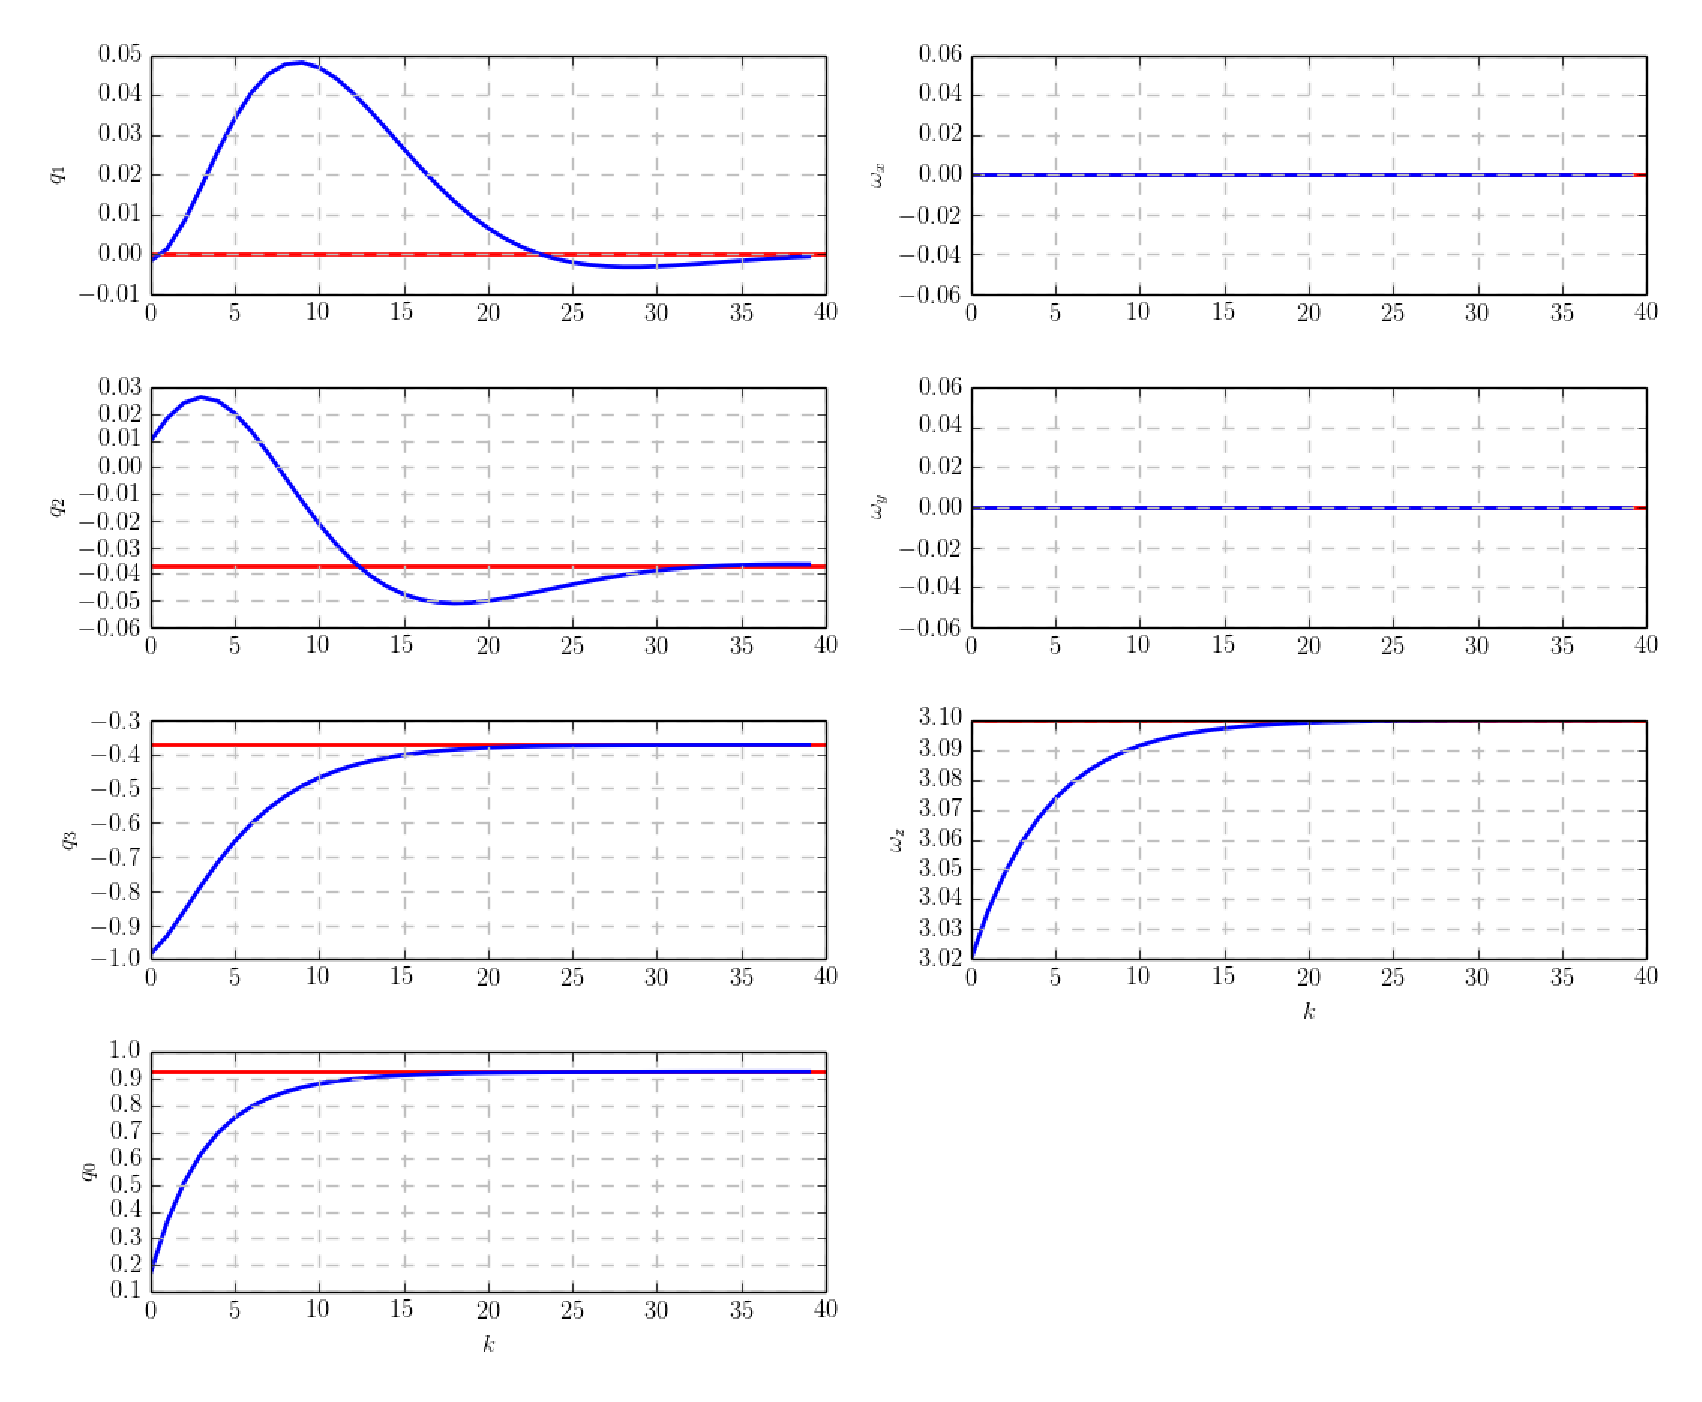
\psfig{file=figures/p_estimator_static_target.eps,width=6in}}
  \caption{P-Estimator with static target}
  \label{fig:PEstimatorwithstatictarget}
\end{figure}

The work covered so far in this chapter has all dealt with the a system in a static state.  In Figure \ref{fig:PEstimatorwithstatictarget}, a P-Estimator converges it's estimated state (blue) to the static measured state (red).  While the estimated state converges to the measured state after about 40 iterations, this type of conversion would be effective only for non-rotating systems.  The non-zero $\omega_z$ means that the quaternion attitude representation will be in constant motion.

The $3.1$ rad/sec rotation about $0\bs{i} + 0.1\bs{j} + 1\bs{k}$ condition from the previous p-estimator is then allowed to propagate the quaternion state through 10 second of rotation with state estimate updates every 0.1 sec.  The resulting measured state (red) and estimated state (blue) is shown in Figure \ref{fig:PEstimatorwithrotatingtarget}.  The body rates track identically to those in Figure \ref{fig:PEstimatorwithstatictarget} where $t(k) = 2$ corresponds to $k = 20$.  Due to the proportional only compensation and no predictive methods, the initial transient behavior is followed by a behavior similar to a steady state error.

\begin{figure}[H]
  \centerline{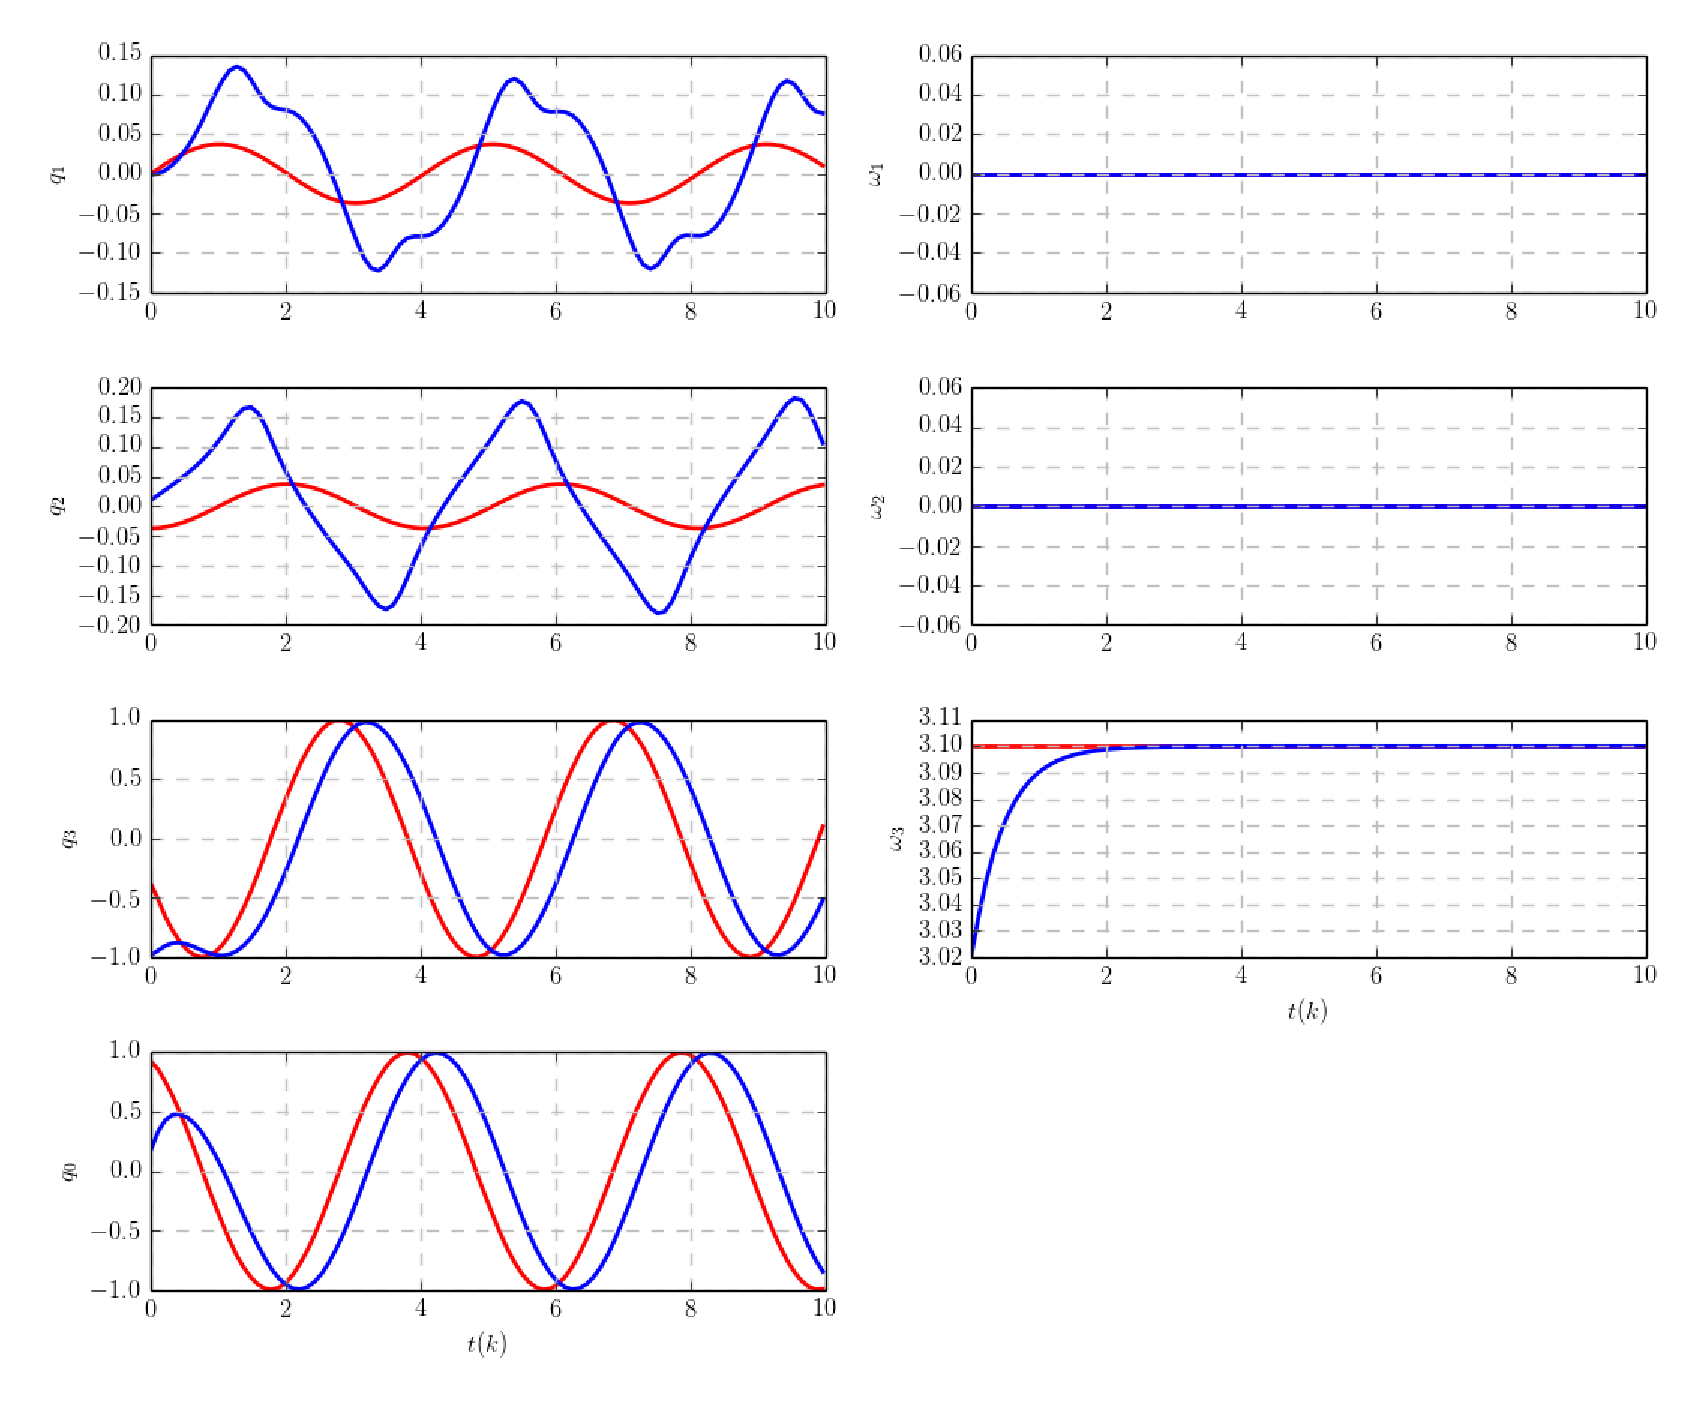
\psfig{file=figures/p_estimator_3radps.eps,width=6in}}
  \caption{P-Estimator with rotating target}
  \label{fig:PEstimatorwithrotatingtarget}
\end{figure}

Increasing the frequency of updates to the p-estimator can decrease the error between the measured and estimated states, but there will always be an error similar to a steady state error in the quaternion representation.  For better results the estimator needs to take into consideration changes in the state through the PID's integration and derivative terms.

\subsubsection{Integral Estimator}
\label{subsubsec:IntegralEstimator}

To stay consistent with the findings in the State Error section (\ref{sec:StateError}), the quaternion portion of the integrated state should abide by the quaternion multiplicative correction method.  This is the first model where the variable sized time step is also taken into consideration.  Instead of accumulating the error measurements, the error corrections should be weighted according to the length of time between updates $t(k+1) - t(k)$.  In a simplified case the integral term should end up the same in the following two update instances.

\begin{table}[H]
  \centering
  \begin{tabular}{r|c|c|c|c|c}
    $t_1 (sec)$ & 0.1 & 0.2 & 0.3 & 0.4 & 0.5 \\ \hline
    $\theta_e$ & 4 & -3 & -3 & -3 & 5 \\
    \\
    $t_2 (sec)$ & 0.1 & & & 0.4 & 0.5 \\ \hline
    $\theta_e$ & 4 &  &  & -3 & 5 \\
  \end{tabular}
  \label{tbl:VariableUpdates}
\end{table}

In $t_1$, regular updates occur every 0.1 sec ending in an integral error value of 0.  In $t_2$, without taking into consideration the variable step sizes would end in an error value of $+6$, but really the -3 error update should be worth three times as much.

Running the state estimator without compensating for variations in time step sizes can create inconsistencies between different experimental runs.  In Figure \ref{fig:IEstimatorwithouttimevariationcompensation}, the integral estimator was updated with a fixed state for 30 seconds.  The estimator was initialized at $0$ radians and run three times against a fixed angle of $0.5$ radians.  The first time with an estimation update frequency of every 0.4 seconds (blue), second with the update frequency of every 0.1 seconds (red), and third with a variable update frequency (green) that jumped back and forth between updating every 0.05 and 0.4 seconds.

\begin{figure}[H]
  \centerline{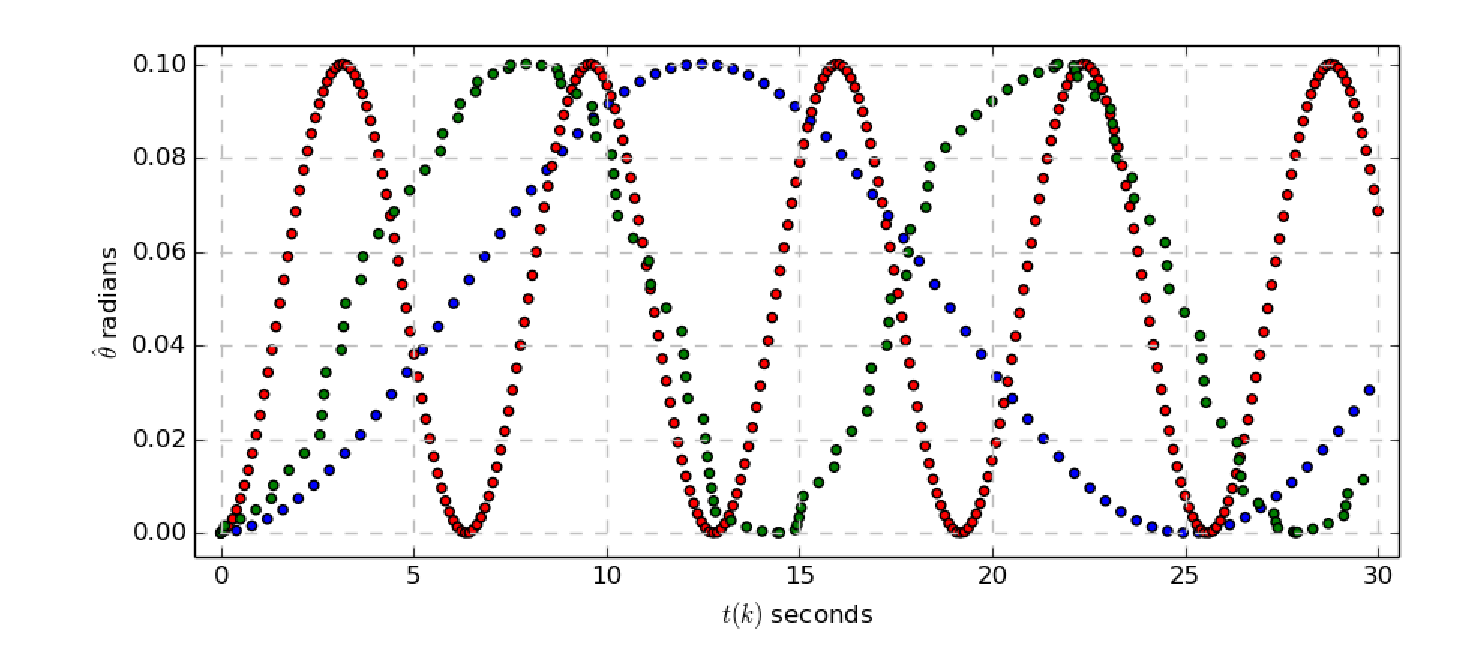
\psfig{file=figures/i_estimator_no_time_varying.eps,width=6in}}
  \caption{I-Estimator without time variation compensation}
  \label{fig:IEstimatorwithouttimevariationcompensation}
\end{figure}

Each calculated estimate for $\hat{\theta}$ in the $k$ domain is identical for each of the three runs, but varies greatly in the time domain.  Most notably, the third run that alternates between update frequencies ends up creating an estimation dynamic that could make the controller less robust.

In comparison, the PID estimator was modified to incorporate the time step size into it's integral term.  The same three tests were run as above with the 0.1 (red), 0.4 (blue), and variable 0.05/0.4 (green) time steps.  The adjustment quaternion method from Section \ref{subsec:RepresentativeStateAdjustments} is first used to compensate for measured time step size of $\Delta t_{k}$ creating a consistent error quaternion. then is used as before to scale the error quaternion by the selected gain value.  The results of this work can be seen in Figure \ref{fig:IEstimatorwithtimevariationcompensation} where the three test runs are still not identical, but their dynamics are more similar than before.  More notably, the variable step test (green) shows less variability in the estimate being produced which will reduce the noise being transferred to the control algorithm.

\begin{subequations}
  \begin{align}
    \bs{\hat{x}}(t_{k+1}) &= \begin{bmatrix} \bs{\hat{q}}(t_{k+1}) \\ \bs{\hat{\omega}}(t_{k+1}) \end{bmatrix} \\
    \bs{\hat{q}}(t_{k+1}) &= \bs{\psi}\big(\bs{q}_{ei}(t_k), K_{qi}\big) \otimes \bs{\hat{q}}(t_{k}) \\
    \bs{q}_{ei}(t_k) &= \bs{\psi}(\bs{q}_e(t_{k}), \Delta t_{k}) \otimes \bs{q}_{ei}(t_{k-1})\\
    \bs{\hat{\omega}}(t_{k+1}) &= \bs{\hat{\omega}}(t_{k}) + \bs{K}_{\omega i} \cdot (\Delta t_k \bs{I})\cdot \bs{\omega}_e(t_{k})
  \end{align}
  \label{eqn:IEstimator}
\end{subequations}

In Equation \ref{eqn:IEstimator}, the error quaternion $\bs{q}_{ei}(t_k)$ used is an accumulation of the time step scaled errors encountered in all previous steps.  This is analogous to a running summation of the error values.  For the body rate estimation, it's largely the traditional integral component with an extra $\Delta t_k \bs{I}$ term that linearly scales the body rate error calculations based on the size of the current time step.

\begin{figure}[H]
  \centerline{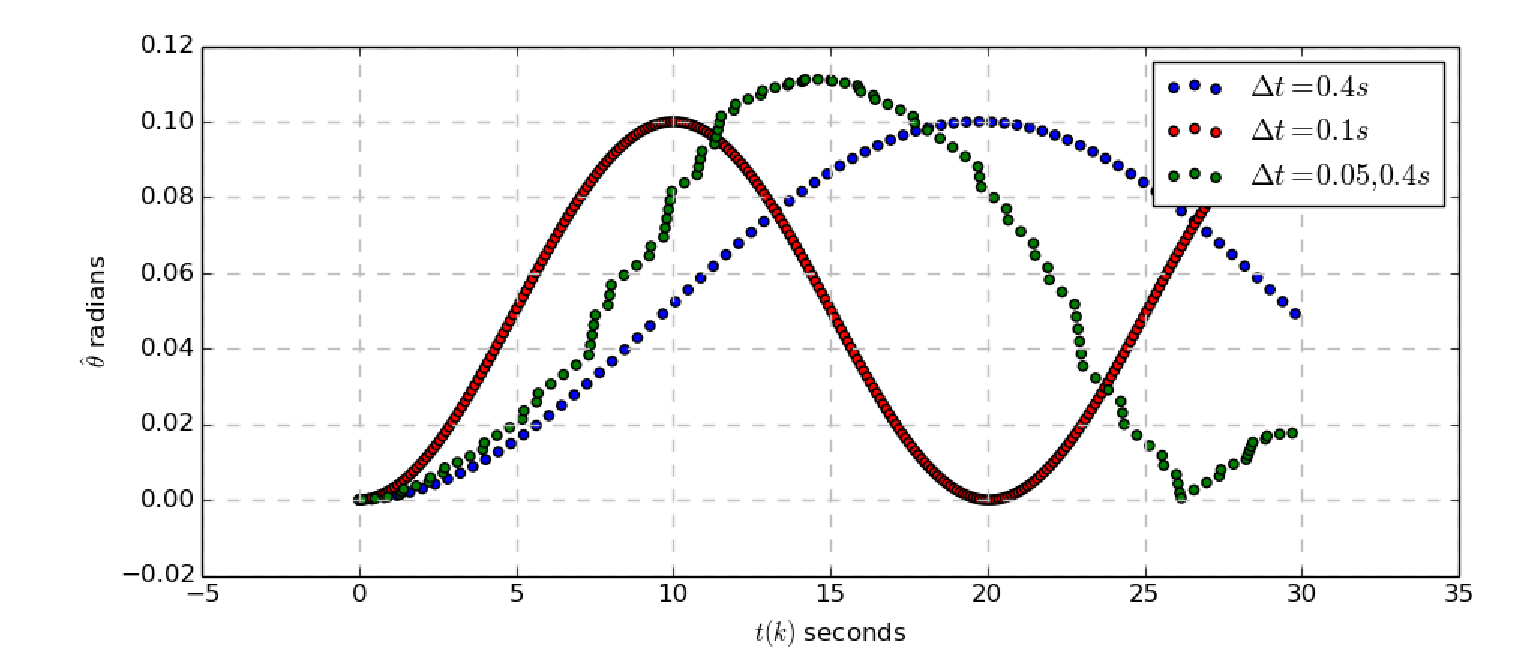
\psfig{file=figures/i_estimator_time_varying.eps,width=6in}}
  \caption{I-Estimator with time variation compensation}
  \label{fig:IEstimatorwithtimevariationcompensation}
\end{figure}

\subsubsection{Derivative Estimator}
\label{subsubsec:DerivativeEstimator}

The derivative component of the PID estimator takes a similar form to the integral component in Equation \ref{eqn:IEstimator}.  The derivative component is only concerned with the current error, previous error, and the current time step size.  As with the integral body rate correction, the derivative correction is scaled by $\frac{1}{\Delta t_k}$ to compensate for variable step sizes.

\begin{subequations}
  \begin{align}
    \bs{\hat{x}}(t_{k+1}) &= \begin{bmatrix} \bs{\hat{q}}(t_{k+1}) \\ \bs{\hat{\omega}}(t_{k+1}) \end{bmatrix} \\
    \bs{\hat{q}}(t_{k+1}) &= \bs{\psi}\left(\bs{q}_{ed}(t_k), K_{qd}\right) \otimes \bs{\hat{q}}(t_{k}) \\
    \bs{q}_{ed}(t_k) &= \bs{\psi}\left(\bs{q}_e(t_{k-1})^* \otimes \bs{q}_e(t_{k}), \frac{1}{\Delta t_{k}}\right)\\
    \bs{\hat{\omega}}(t_{k+1}) &= \bs{\hat{\omega}}(t_{k}) + \bs{K}_{\omega d} \cdot \left(\frac{1}{\Delta t_k} \bs{I}\right) \cdot \bs{\omega}_e(t_{k})
  \end{align}
  \label{eqn:DEstimator}
\end{subequations}

The Figures \ref{fig:DEstimatorwithouttimevariationcompensation} and \ref{fig:DEstimatorwithtimevariationcompensation} below are the results of three test runs with the same set up update frequencies as with the integral component (0.1/sec, 0.4/sec, and varied).  For this comparison, the TableSat was simulated into a steady $0.01$ rad/s rotation about the body $+z$-axis to generate a constant rate of change for the quaternion instead of the fixed quaternion in the integral test.  The $\theta_{adj}$ parameter tracked for this test is the angular rotation associated with the $\bs{\psi}\left(\bs{q}_{ed}(t_k), K_{qd}\right)$ quaternion adjustment term.

\begin{figure}[H]
  \centerline{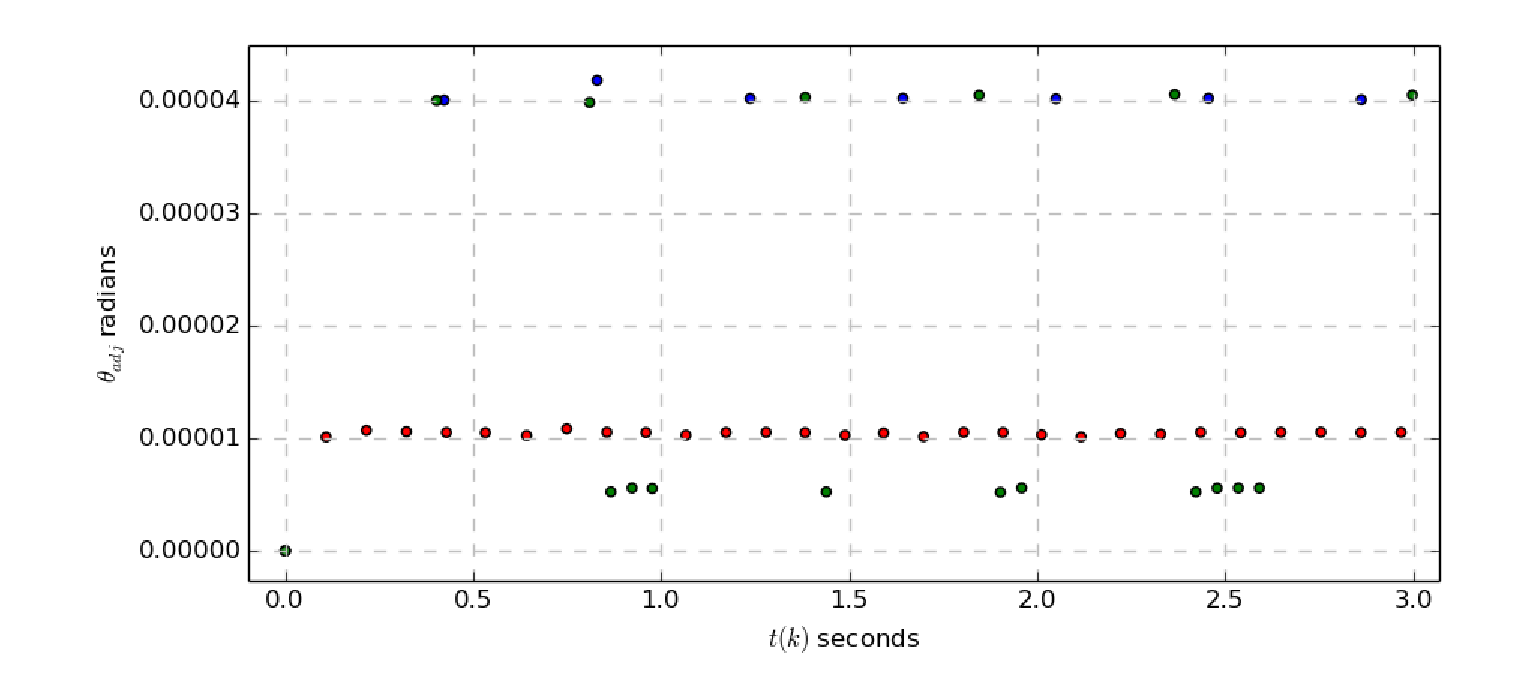
\psfig{file=figures/d_estimator_no_time_varying.eps,width=6in}}
  \caption{D-Estimator without time variation compensation}
  \label{fig:DEstimatorwithouttimevariationcompensation}
\end{figure}

Figure \ref{fig:DEstimatorwithouttimevariationcompensation} shows the results of the test run without consideration taken for time step sizes.  With a constant spin rate, the resulting quaternion adjustment is tightly coupled to the frequency that the updates are made with the 0.1 (red), 0.4 (blue), and variable 0.05/0.4 (green) time steps.  The variable time step sequence is a particular concerns as it jumps back and forth between adjusted amount suggesting the spin rate is not constant.

\begin{figure}[H]
  \centerline{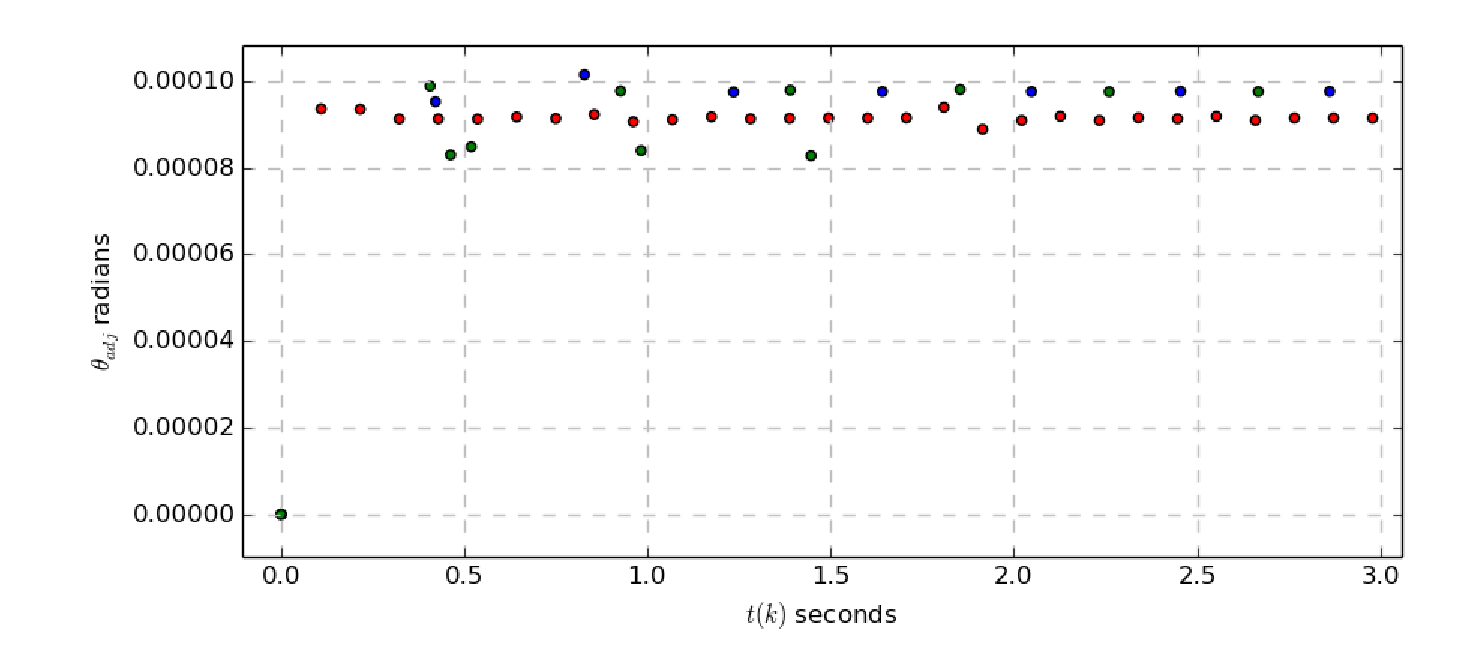
\psfig{file=figures/d_estimator_time_varying.eps,width=6in}}
  \caption{D-Estimator with time variation compensation}
  \label{fig:DEstimatorwithtimevariationcompensation}
\end{figure}

Figure \ref{fig:DEstimatorwithtimevariationcompensation} implements the time variation compensation in Equation \ref{eqn:DEstimator} where the quaternion adjustments provide a better representation of the measured constant spin rate.

\subsubsection{PID Estimation of Unforced Motion}
\label{subsubsec:PIDEstimatorofUnforcedMotion}

Combining the proportional, integral, and derivative estimator portions from above.  Equations \ref{eqn:PEstimator}, \ref{eqn:IEstimator}, and \ref{eqn:DEstimator} get combined into a single PID estimator as

\begin{subequations}
  \begin{align}
    \bs{\hat{x}}(t_{k+1}) &= \begin{bmatrix} \bs{\hat{q}}(t_{k+1}) \\ \bs{\hat{\omega}}(t_{k+1}) \end{bmatrix} \\
    \bs{\hat{q}}(t_{k+1}) &= \bs{\psi}\left(\bs{q}_{ed}(t_k), K_{qd}\right) \otimes \bs{\psi}\big(\bs{q}_{ei}(t_k), K_{qi}\big) \otimes \bs{\psi}(\bs{q}_e(t_{k}), K_{qp})  \otimes \bs{\hat{q}}(t_{k}) \\
    \bs{\hat{\omega}}(t_{k+1}) &= \bs{\hat{\omega}}(t_{k}) + \bs{K}_{\omega p} \cdot \bs{\omega}_e(t_{k}) + \bs{K}_{\omega i} \cdot (\Delta t_k \bs{I})\cdot \bs{\omega}_e(t_{k}) + \bs{K}_{\omega d} \cdot \left(\frac{1}{\Delta t_k} \bs{I}\right) \cdot \bs{\omega}_e(t_{k})
  \end{align}
  \label{eqn:PIDEstimatorUnforcedMotion}
\end{subequations}

The update to the estimated body rate follows the traditional method of the PID control with the addition of the scaling factors for the integral and derivative terms that compensate for non-uniform step sizes at run-time.  The quaternion correction is a compilation of the individual correction quaternions and joined through the multiplicative error correction method.

With a spin stabilized system controlling the body rate is relatively straight forward with a PID controller.  A test was run through TSatPy with based on the PID estimation in Equation \ref{eqn:PIDEstimatorUnforcedMotion}.  The system was set at a spin rate of $0.314$ rad/sec rotation about $+z$ with the measurement of the quaternion angle $\theta$ containing noise $N \sim (0, 0.1218)$ radians.  A gradient descent gain selection settled on the following parameters.

\begin{equation}
  \begin{aligned}
    K_{qp} &= 0.98, K_{qi} = 0.001, K_{qd} = 0.001 \\
    \bs{K}_{\omega p} &= 0.7 \bs{I}, \bs{K}_{\omega i} = \bs{0}, \bs{K}_{\omega d} = \bs{0}
  \end{aligned}
\end{equation}

The test run results are show in Figure \ref{fig:PIDEstimatorwithoutstateprediction}.  The bottom two graphs showing body rate tracking performance where the basic proportional control quickly brings the body rate error under control.  The quaternion estimations are much more difficult largely due to the lack of a system model to convert body rates to estimated attitudes at the next update.  Since the system is spin stabilized and the estimated quaternion has no prior knowledge of where the next value will be, it relies on a large proportional component to jump to the new measurement values on each update.

While testing the performance of the integral and derivative components showed an improved performance when incorporating the effects of the variable time step, in this test with such a heavy reliance on the proportional component, the benefits to considering the variable time step effects were negligible.

\begin{figure}[H]
  \centerline{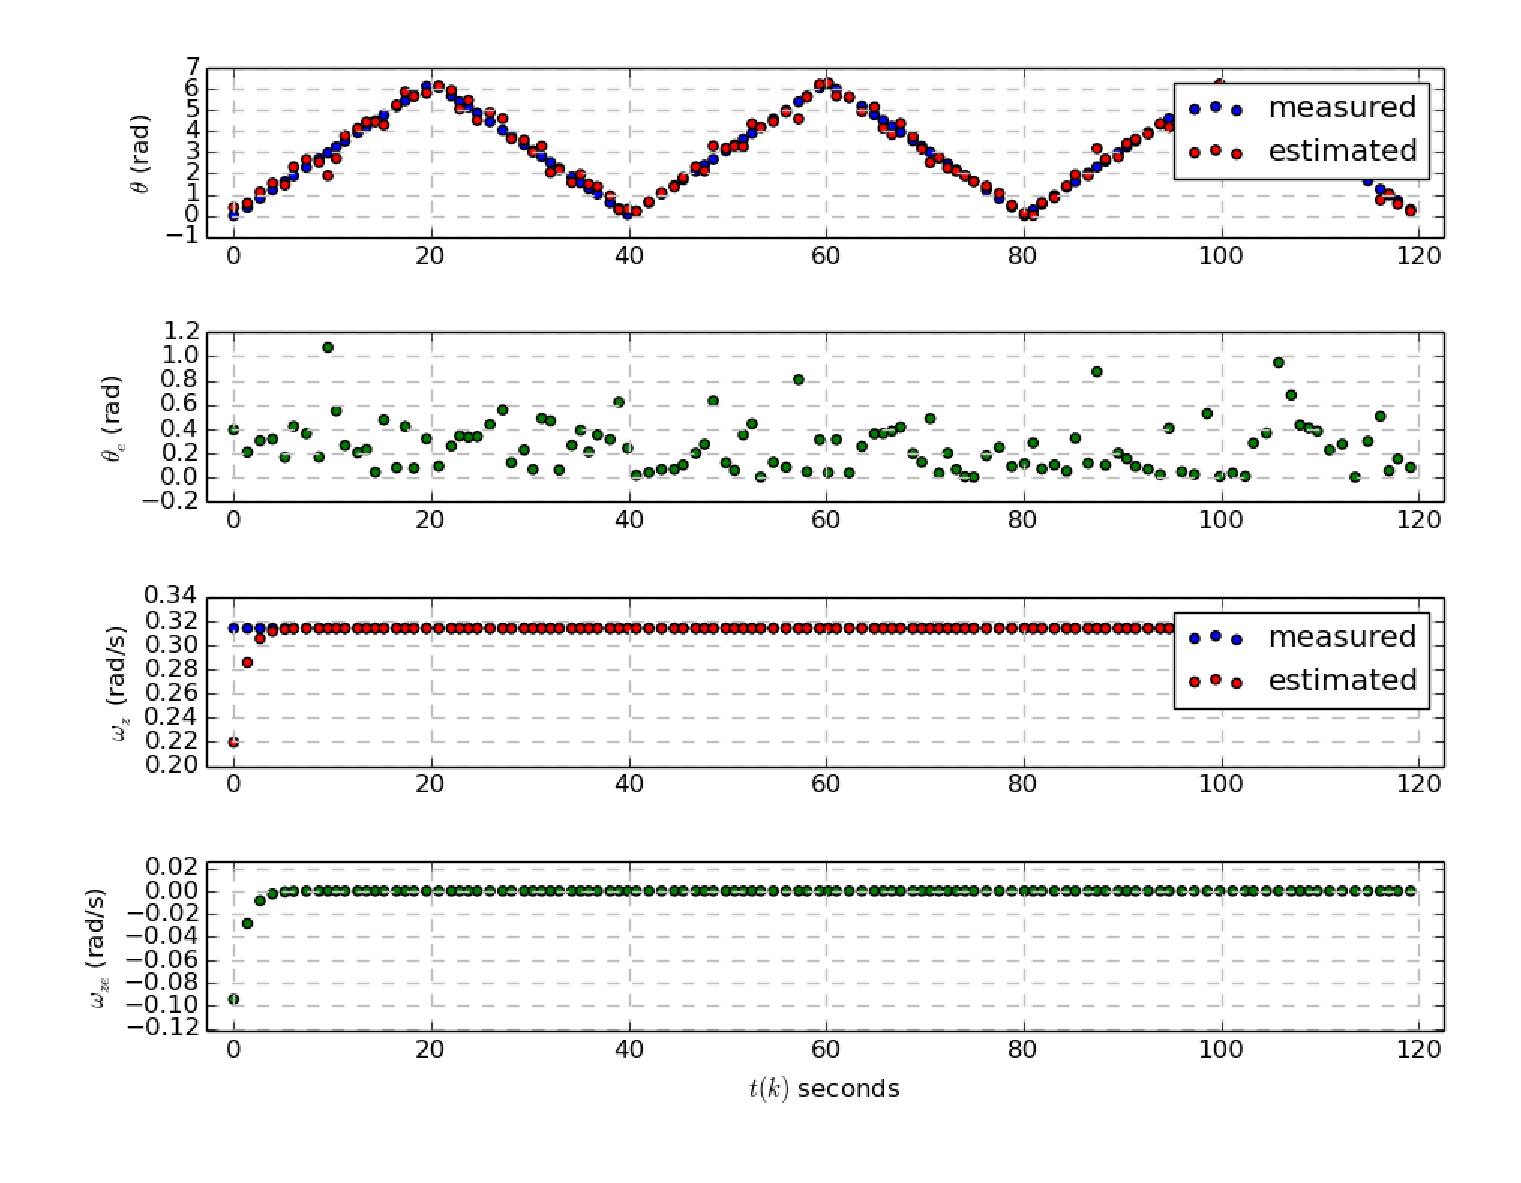
\psfig{file=figures/pid_estimator_no_prediction_high_P.eps,width=6in}}
  \caption{PID-Estimator without state prediction}
  \label{fig:PIDEstimatorwithoutstateprediction}
\end{figure}

\subsection{State Prediction}
\label{subsec:StatePrediction}

Section \ref{subsec:PIDEstimation} shows that to keep accurate tracking of a spin stabilized satellite like TableSat or MMS, the system's dynamic equations are required to couple the body rate and quaternion values.  This is especially important for the TableSat 1A implementation since only the magnetometer and course sun sensors provide feedback about the system's state, and they only have a partial measurement of the attitude quaternion and no direct measurement of the body rates.

The approach taken in the TSatPy code to create state predictions off previous state estimates is to start with a discretized Euler's Moment Equations \ref{eqn:DiscreteEulerMomentEquations} to predict $\bs{\dot{\omega}}(t_{k+1})$.  The the current estimated body rate is adjusted based on the variable time step size.

\begin{equation}
  \bs{\omega}(t_{k+1}) = \bs{\omega}(t_{k}) + \bs{\dot{\omega}}(t_{k+1})\cdot (t_{k+1} - t_k)
\end{equation}

The newly estimated body rates $\bs{\omega}(t_{k+1})$ are supplied to the discretized quaternion dynamics Equation \ref{eqn:DiscreteQuaternionPropagation} to calculate the newly estimated rotational quaternion.

\subsection{PID Estimation with State Prediction}
\label{subsec:PIDEstimatorwithStatePrediction}

From Section \ref{subsec:PIDEstimation}, Equation \ref{eqn:PIDEstimatorUnforcedMotion} defines a method of tracking unforced spin stabilized satellites through PID state estimation.  The biggest issue was a heavy reliance on the proportional gain to track the quaternion attitude which is sensitive to measurement noise.  Incorporating a multiplicative-correction quaternion based model of rigid body dynamics based on the equations in Chapter \ref{chap:SatelliteAttitudeModeling} can assist in predicting the $t_{k+1}$ state of the system.

\begin{subequations}
  \begin{align}
    \bs{\hat{x}}(t_{k+1}) &= \begin{bmatrix} \bs{\hat{q}}(t_{k+1}) \\ \bs{\hat{\omega}}(t_{k+1}) \end{bmatrix} \\
    \bs{\hat{q}}(t_{k+1}) &= \bs{\psi}\left(\bs{q}_{ed}(t_k), K_{qd}\right) \otimes \bs{\psi}\big(\bs{q}_{ei}(t_k), K_{qi}\big) \otimes \bs{\psi}(\bs{q}_e(t_{k}), K_{qp})  \otimes \bs{\hat{q}}(t_{k+1})^- \\
    \bs{\hat{\omega}}(t_{k+1}) &= \bs{\hat{\omega}}(t_{k+1})^- + \bs{K}_{\omega p} \cdot \bs{\omega}_e(t_{k}) + \bs{K}_{\omega i} \cdot (\Delta t_k \bs{I})\cdot \bs{\omega}_e(t_{k}) + \bs{K}_{\omega d} \cdot \left(\frac{1}{\Delta t_k} \bs{I}\right) \cdot \bs{\omega}_e(t_{k})
  \end{align}
  \label{eqn:PIDEstimatorwithPredictionUnforcedMotion}
\end{subequations}

with the a priori state $\bs{\hat{x}}(t_{k+1})^-$ as

\begin{equation}
  \bs{\hat{x}}(t_{k+1})^- = \begin{bmatrix}\bs{\hat{q}}(t_{k+1})^- \\ \bs{\hat{\omega}}(t_{k+1})^- \end{bmatrix} = f \Big( \bs{\hat{q}}(t_{k}), \bs{\hat{\omega}}(t_{k}) \Big)
\end{equation}

The PID estimator now with a state prediction method was run under the same testing conditions present in Figure \ref{fig:PIDEstimatorwithoutstateprediction}.  The resulting performance showed that the inclusion of the system model greatly reduced the reliance on the proportional component of the PID estimator which reduced the noise and increased the accuracy of the final estimates being provided to the controller.  The results in Figure \ref{fig:PIDEstimatorwithstateprediction} show the improved quaternion angle estimates when run with the following gains.

\begin{equation}
  \begin{aligned}
    K_{qp} &= 0.0735, K_{qi} = 0.000863, K_{qd} = 0.00812 \\
    \bs{K}_{\omega p} &= 0.7 \bs{I}, \bs{K}_{\omega i} = \bs{0}, \bs{K}_{\omega d} = \bs{0}
  \end{aligned}
\end{equation}

The quaternion's proportional value is still the dominant gain, but has been reduced by 92.5\% of it's previous value while still providing about 80\% reduction in quaternion attitude error rates.

\begin{figure}[H]
  \centerline{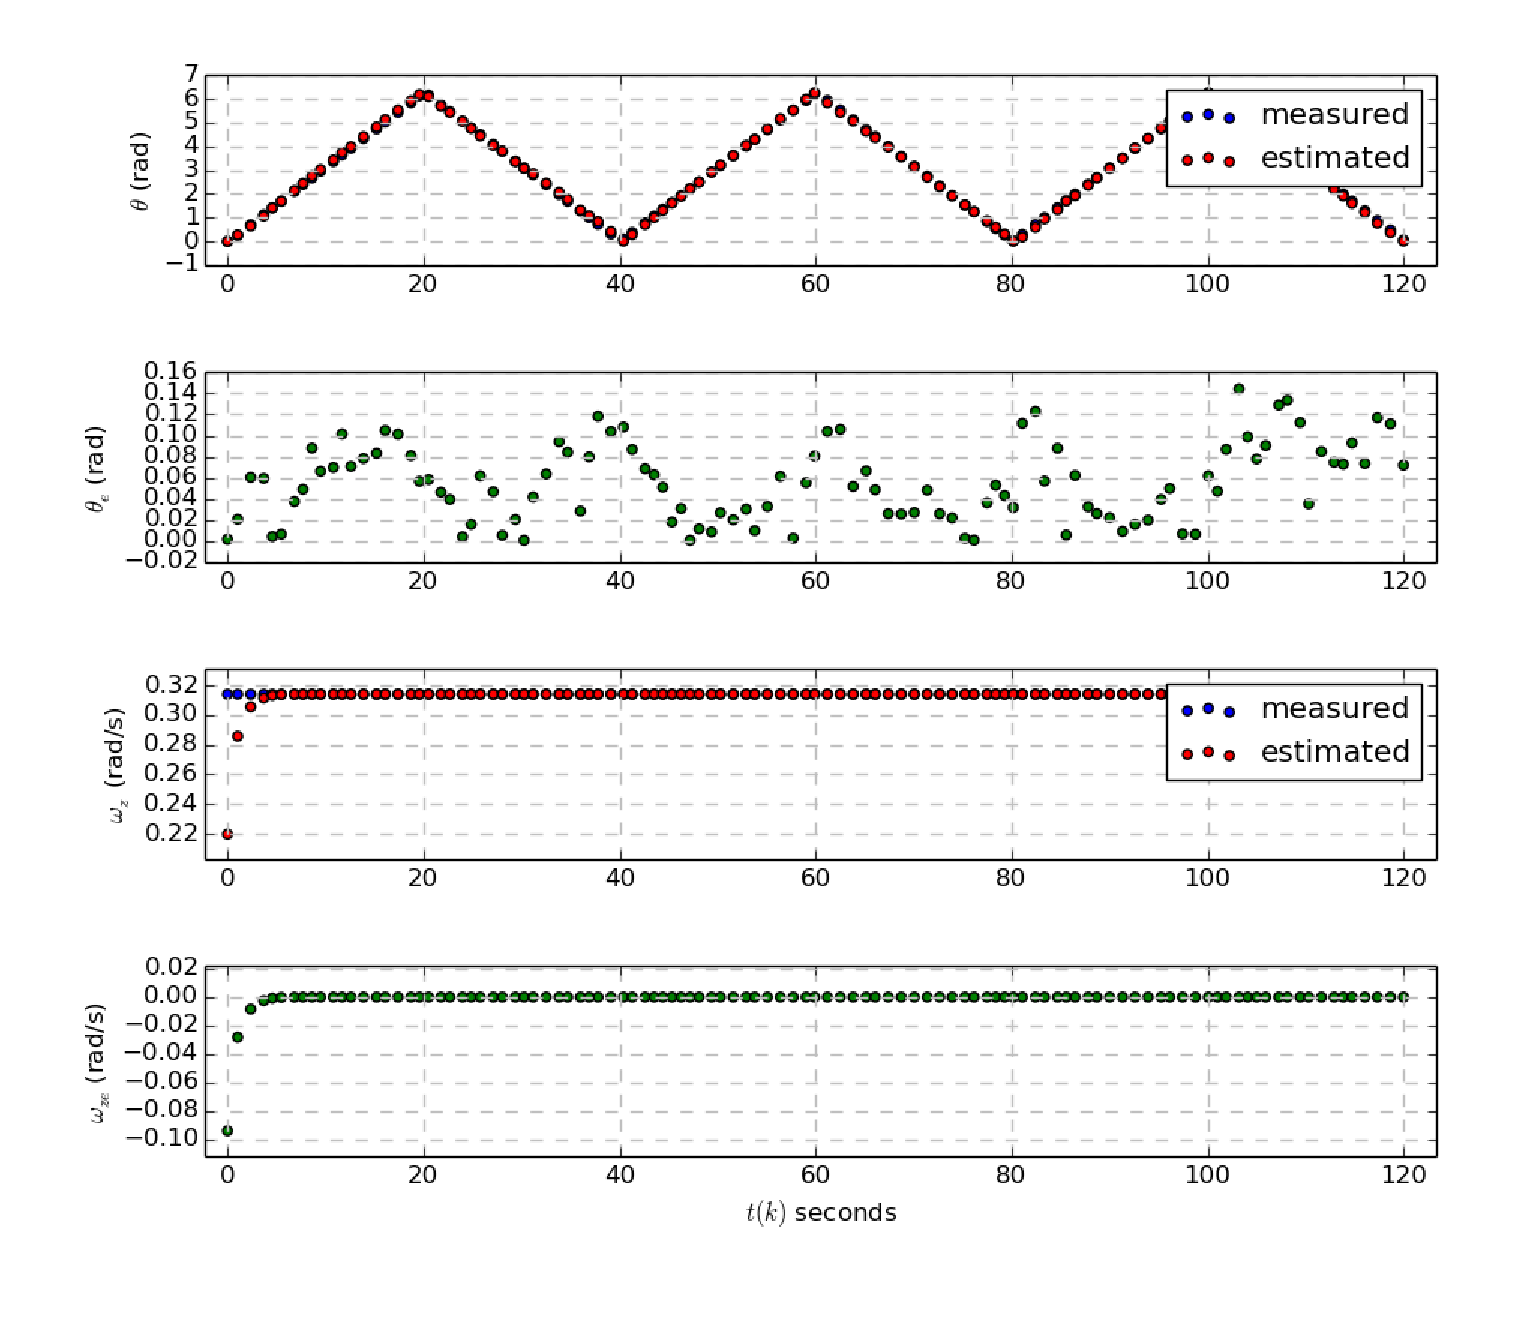
\psfig{file=figures/pid_estimator_with_prediction.eps,width=6in}}
  \caption{PID-Estimator with state prediction}
  \label{fig:PIDEstimatorwithstateprediction}
\end{figure}


\subsection{Sliding Mode Observer}
\label{subsec:SlidingModeObserver}

The Sliding Mode Observer (SMO) is a proportional estimator with an additional smoothing term that uses a chosen sliding surface.  The general form for the SMO is

\begin{equation}
  \bs{\dot{\hat{x}}} = \bs{\hat{f}}(\bs{\hat{x}}, \bs{\hat{u}}, t) + \bs{L}(\bs{C}\bs{\hat{x}} - \bs{C}\bs{x}) + \bs{K}\bs{1}_s\bs{\hat{y}}
  \label{eqn:SMOContinuous}
\end{equation}

Where L is a luenberger gain and $\bs{1}_s$ is a switching function based on $s$.  The sliding mode terms allow additional control of the state adjustments without adding a lot of computational complexity.  The SMO can continue to use the nonlinear model's state predictions as in the PID estimators in Section \ref{subsec:PIDEstimatorwithStatePrediction}, which is an advantage over methods such as the Extended Kalman Filter (EKF) where the system is linearized about an operating point and assumes a constant time step.

This thesis takes the discretized form of Equation \ref{eqn:SMOContinuous} with a quaternion multiplicative correction

\begin{subequations}
  \begin{align}
    \bs{\hat{x}}(t_{k+1}) &= \begin{bmatrix} \bs{\hat{q}}(t_{k+1}) \\ \bs{\hat{\omega}}(t_{k+1}) \end{bmatrix} \\
    \bs{\hat{q}}(t_{k+1}) &= \bs{1}_s\big(\bs{q}_{e}(t_k)\big) \otimes \bs{\psi}(\bs{q}_e(t_{k}), L_{q})  \otimes \bs{\hat{q}}(t_{k+1})^- \\
    \bs{\hat{\omega}}(t_{k+1}) &= \bs{\hat{\omega}}(t_{k+1})^- + \bs{L}_{\omega} \bs{\omega}_e(t_{k}) + \bs{1}_s \big(\bs{\omega}_e(t_{k}) \big)
  \end{align}
  \label{eqn:PIDEstimatorwithPredictionUnforcedMotion}
\end{subequations}

where

\begin{subequations}
  \begin{align}
    \bs{1}_s\big(\bs{q}_{e}(t_k) \big) &= \begin{bmatrix} \bs{v_e} \\ sat\left( \frac{\cos^{-1} q_{0e} }{S_{q}} \right) \end{bmatrix} \\
    \bs{L}_{\omega} &= L_\omega \cdot \bs{I} \\
    \bs{1}_s \big(\bs{\omega}_e(t_{k}) \big) &= sat\left( \frac{\bs{\omega}_e(t_{k})}{S_{\omega}} \right)
  \end{align}
\end{subequations}

For body rates, the a priori state provides the predicted body rate $\bs{\hat{\omega}}(t_{k+1})^-$ that gets adjusted by a proportional term $\bs{L}_{\omega} \bs{\omega}_e(t_{k})$ as in the P-Estimator, but has an additional saturation function correction based on sliding surfaces for the individual body rate errors.  As found in the PID estimator, the proportional estimator for a steady spin stabilized satellite performs adequately.  The additional saturation term becomes helpful for situations with low $L_\omega$ values that can take longer to converge from the initial body rate to the actual body rate, but once close will increase the effort in staying in step with the measured body rate.

Similar to the PID estimator, the quaternion sliding mode observer limits it's focus to the angular measure of the rotational quaternion.  The sliding surface is taken based on the radian measure.  If the radian measure is below, the saturation limit the quaternion stays as is.  If the quaternion represents a rotation greater than the saturation limit a saturated quaternion is created about the same Euler axis but limit to the saturation angle of rotation.

kwargs = {'S': {'q': 1.908376120345185, 'w': 6.5356517995605596}, 'K': {'q': 0.12520202719936652, 'w': 0.48433605036767613}, 'L': {'q': 0.41506774287666348, 'w': 0.35072151415483038}}
kwargs = {"S": {"q": 0.7324366102332057, "w": 0.5386880719560759}, "K": {"q": 0.6340430770694714, "w": 0.5821736289388915},  "L": {"q": 0.7814360951486294, "w": 0.736085136529068}}

\begin{figure}[H]
  \centerline{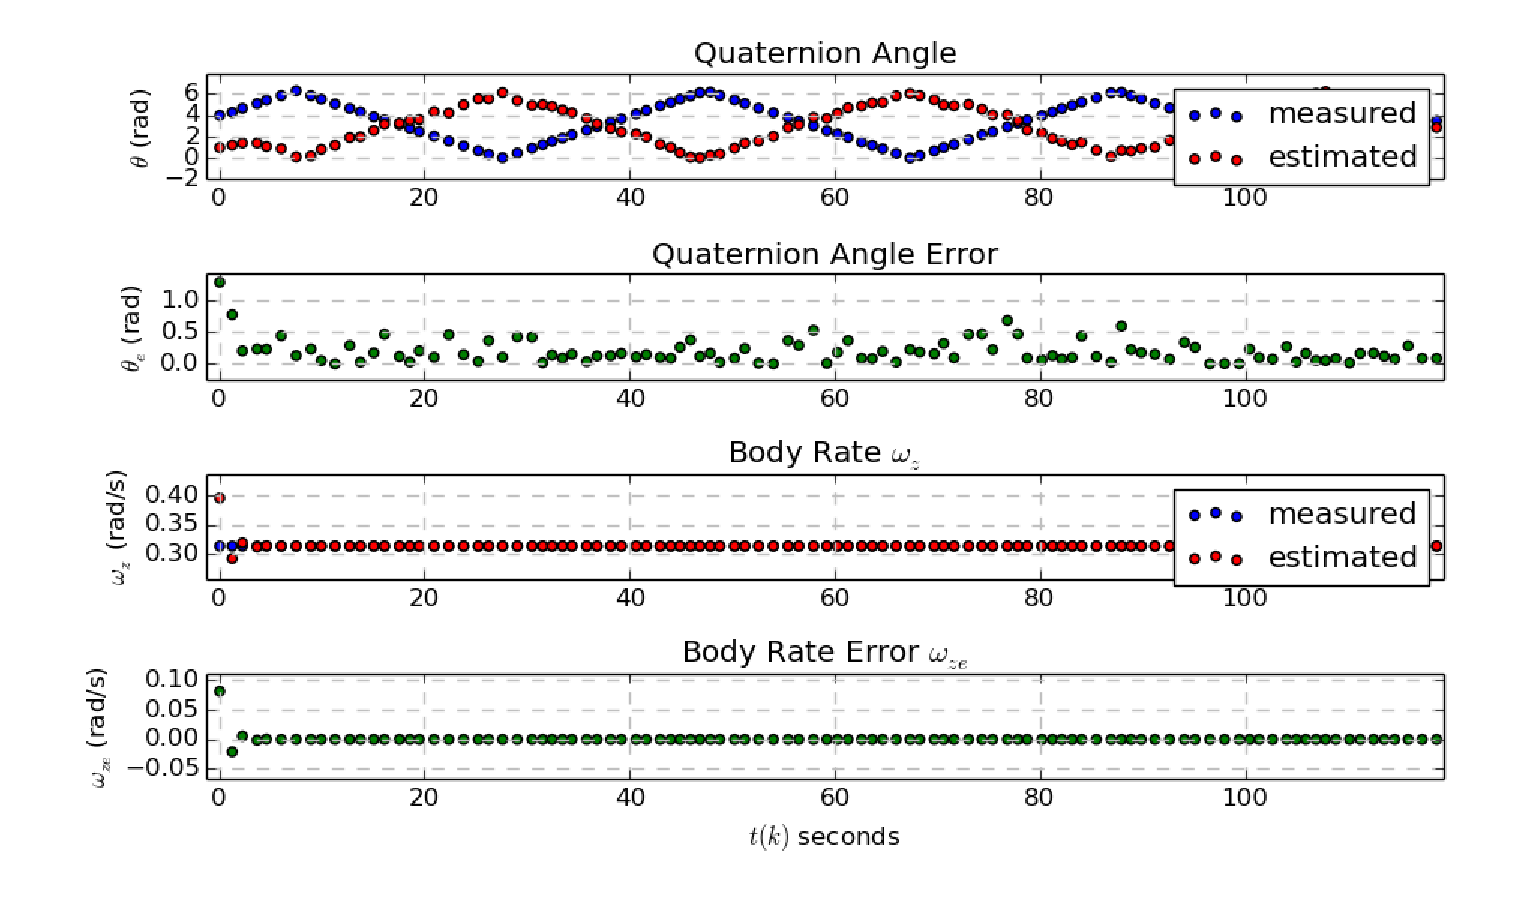
\psfig{file=figures/smo_estimator_with_prediction.eps,width=6in}}
  \caption{SMO-Estimator with state prediction}
  \label{fig:SMOEstimatorwithstateprediction}
\end{figure}
\begin{figure}[H]
  \centerline{\psfig{file=figures/smo_bad_estimator_with_prediction.eps,width=6in}}
  \caption{SMO-Estimator high gain with state prediction}
  \label{fig:SMOEstimatorhighgainwithstateprediction}
\end{figure}



\section{Controllers}
\label{sec:Controller}
From the MMS requirements, the body rate portion of the desired state is taken as a 3rpm (0.31416 rad/sec) rotation about the satellite's $z$-axis with zero body rates about the $x$ and $y$ axes.

\begin{equation}
  \bs{\omega}_d = \begin{bmatrix} 0 & 0 & 0.31416 \end{bmatrix}^T
  \label{eqn:DesiredBodyRate}
\end{equation}

Since the satellite is spin stabilized, the desired quaternion is not as straight forward.  With a goal of keeping the body's $z$-axis aligned with the global reference frame's $z$-axis the $q_3$ and $q_0$ quaternion values should be allowed to vary as $q_1$ and $q_2$ should remain at zero if no nutation exists.

\begin{equation}
  \bs{q}_d = 0 \bs{i} + 0 \bs{j} + q_3 \bs{k} + q_0
  \label{eqn:DesiredQuaternion}
\end{equation}

\subsection{Quaternion Decomposition}
\label{subsec:QuaternionDecomposition}

\section{Simulations}
\label{sec:Simulations}

\section{Experimental Validation}
\label{sec:ExperimentalValidation}
